% enaR: Tools for Ecological Network Analysis
% Target: Methods in Ecology and Evolution
% October 2013
% ---------------------------------------------------
\documentclass[11pt]{article}
\usepackage[super, sort]{natbib}
  \bibpunct{(}{)}{;}{a}{,}{,} % required for natbib
\bibliographystyle{mee}

\usepackage[margin=1in]{geometry}

\usepackage{amsmath,amssymb,amsthm,amsfonts}
\usepackage[]{graphicx}
\usepackage{setspace} 
\usepackage{lineno} %numbers lines
\usepackage{qtree} %draw tree structures
\usepackage{url}

% --- SRB Defined functions ----
\newcommand{\ppr}{\lambda_1(\mathbf{A})}
\newcommand{\ID}{I/D}
\newcommand{\g}{\lambda_1(\mathbf{G})}
\DeclareMathOperator{\diag}{diag}
\def\citeapos#1{\citeauthor{#1}'s (\citeyear{#1})}
\newcommand{\R}{R}
%\newcommand{\S}{S}
\newcommand{\enaR}{\texttt{enaR}}
\newcommand{\vnorm}[1]{\left|\left|#1\right|\right|}
\newcommand{\midtilde}{\raisebox{-0.25\baselineskip}{\textasciitilde}}
\def\tableline{\vskip .1in \hrule height 0.6pt \vskip 0.1in}
% ----------------
\usepackage[ pdfauthor={Stuart R. Borrett},
pdfkeywords={ecological network analysis, network environ analysis},
pdfpagemode=UseOutlines, bookmarks=T, colorlinks,
linkcolor=blue,citecolor=blue, pdfstartview=FitH,
urlcolor=red]{hyperref}

% ---- FRONT MATTER -----

\title{\enaR: An \R\ package for Ecological Network Analysis}
\author{Stuart R. Borrett$^{a,*}$ and Matthew K. Lau$^b$ \\
 {\footnotesize $^a$ Department of Biology and Marine Biology, University of North
Carolina Wilmington, Wilmington, NC, 28403} \\
 {\footnotesize $^b$ Department of Biological Sciences, Northern Arizona
  University, 617 S.\ Beaver St., Flagstaff, AZ, 86011} \\
 {\footnotesize $^*$ Corresponding author, borretts@uncw.edu}
}

% ------------------------
\begin{document}
\maketitle

\begin{spacing}{2}
\linenumbers

\tableline
\section*{Abstract}
Network ecologists apply network models and analyses to investigate
the structure, function , and evolution of ecological systems.
Ecological Network Analysis (ENA) is an approach rooted in ecosystem
ecology with over 30 years of development.  While some software tools
exist to assist ecologists with the application of ENA, they vary in
their comprehensiveness, availability, usability, transparency, and
extensibility.  Here, we introduced \enaR\, a professional grade set
of \R\ tools that enables ecologist to perform a broad set of ENA
algorithms.  In addition to the basic functionality of the package, we
highlight several values added features including the ability to
visualize the networks, the inclusion of a library of 100
empirically-based ecosystem models, the ability to batch apply the
analyses, and easily connect to other network analysis and ecological
analysis tools in \R .  We expect this tool to enable more ecologists
to apply ENA methods and contribute to their development.

KEYWORDS: network analysis, ecosystem, social network analysis,
software, network environ analysis, ascendency, input--output
analysis, food web, Ecopath
\tableline

\section{Introduction}
% Network Ecology & its significance
Network Ecology -- the study of ecological systems using network
models and analysis to characterize their structure, function, and
evolution -- is a large and rapidly growing area of ecology.
\citet{borrett14_rise} found that more than 5\% of the ecology and
evolutionary biology papers published in 2012 and indexed by Web of
Science could be classified as Network Ecology.  Likewise,
\citet{ings2009} showed that a notable fraction of 2008 publications
in 11 select journals were related to food webs ($\approx$2.4\%),
mututalitsic networks ($\approx$0.9\%), and host-parasitoid networks
($\approx$0.055\%).  Network ecology is growing in part because
ecology is fundamentally a relational science and network models are
excellent tools for relational analyses.  In addition, this rise of
network ecology contributes to, mirrors, and builds on the more
general development of network sciences \citep{wasserman94,
%  barabasi02, 
barabasi12, borgatti2003network, freeman2004development,
  newman03review}

% what is ENA
Ecological Network Analysis (ENA) is a branch of network ecology that
is rooted in ecosystem ecology \citep{borrett12_netecol}.  It works
like a ``macroscope'' to investigate (1) whole system organization,
(2) the direct and indirect effects among system components, and (3)
the processes that create and sustain ecological systems.  More
specifically, ENA is a family of algorithms that are an ecological
application and extension of Leontief's (\citeyear{leontief66})
economic Input-Output Analysis.  These algorithms are applied to
network models of energy and matter exchange among ecosystem
components \citep{patten76, ulanowicz86, fath99_review, hannon73}.


% Two School's: Ulanowicz & Patten
While many influences combined to create what we now call ENA
\citep[e.g.,][]{patten59, margalef63, hannon73, pimm82,
  golley1993history}, since the 1970s two primary schools of thought
have developed \citep{scharler09comparing}.  The
first is based on the work of Dr.\ Robert E. Ulanowicz, which was
centered at the University of Maryland \citep{ulanowicz86,
  ulanowicz97, ulanowicz09_window}.  The Ulanowicz school of ENA is
primarily focused on trophic ecology, and its starting point is a
phenomenological map of the energy--matter exchanges among ecosystem
components.  A key contribution of this work is the use of information
theory and the development of the ascendecy concept that
\citet{ulanowicz86, ulanowicz97} used to characterize ecosystem growth
and development.  The second school is based on the work of Dr.\
Bernard C. Patten at the University of Georgia \citep{patten76,
  matis81, patten82, fath99_review}.  Its initial perspective was
steeped in dynamic equations, simulations, and systems analysis, with
a distinct network flavor.  A key contribution of this work is the
environ concept that formalizes the concept of environment for study
inside the network models \citep{patten78}.  The Patten School of work
has often been referred to as ``Network Environ Analysis''.  The
Ulanowicz and Patten School's of ENA represent two distinct but
interwoven developments.  Together, they join information theory,
environmental concepts, and network science to study ecosystems.

% examples of recent use
The development of ENA has contributed to a new theoretical
understanding of ecosystems \citep{ulanowicz86, higashi91, belgrano05,
  jorgensen07_newecology} and the techniques have been applied in a
multiple ways.  For example, \citet{patten82} used a storage analysis
to identify two nearly separate hydrologic subsystems in the
Okefenokee Swamp, USA.  \citet{bondavalli99} showed that in the
Florida Everglades the American alligator is an indirect mutualist
with several of its prey, including frogs.  \citet{hines12} used
ENA to study the Cape Fear River estuary sediment nitrogen cycle, and applied
the tools to quantify the coupling between biogeochemical processes
(e.g., nitrification + anammox).  
%Subsequent work showed the potential
%impact of sea water intrusion on the N cycle \citep{hines14}. % this
                                % hines text is clunky.  
Furthermore, several scientists have used ENA to investigate urban
sustainability \citep{bodini02, zhang10_ecomod, chen12,
  bodini2012cities}.  Collectively, this work consistently shows the
power of the interaction network to transform relationships among
system components in non-obvious ways that require whole-systems
analysis to elucidate \citep{ulanowicz90, patten91,
  fath07_netconstruction}.

% Existing Software/Tools : NETWRK, WAND, ECOPATH, NEA.m EcoNet
Several software tools have been created to enable scientists to more
easily apply ENA. The first widely distributed tool was NETWRK
\citep{ulanowicz91}.  This program is a collection of analyses from
the Ulanowicz School that is programmed in Fortran and distributed as
a DOS executable file. Version 4.2 is available from
%(\href{http://www.cbl.umces.edu/~ulan/ntwk/network.html}{http://www.cbl.umces.edu/$\sim$ulan/ntwk/network.html}).
\url{http://www.cbl.umces.edu/~ulan/ntwk/network.html}
WAND is a Microsoft Excel based re-implementation of many but not all
of the algorithms in NETWRK \citep{allesina04_wand}. An explicit goal
of WAND was to be more accessible for ecologists, who have tended to
be more familiar with Excel than DOS.  \citet{fath06} introduced a
Matlab function, NEA.m, that assembled the primary algorithms from the
Patten School.  One advantage of NEA.m is that the algorithms are
transparent to the user and accessible for modification.  While the
NEA.m function is freely available
(\url{http://www.mathworks.com/matlabcentral/fileexchange/5261-nea-m})
%{http://www.mathworks.com/matlabcentral/fileexchange/5261-nea-m})
it requires Matlab, which is a powerful but expensive program.  With
modification, the function can be run in Octave, an open source clone
of Matlab, but it executes more slowly.  EcoNet is a web-based tool
that lets users apply ENA primarily from the Patten School, but with
some computational enhancements \citep{kazanci07, schramski11}.
Ecopath with Ecosim \citep{christensen92, christensen04} is used
primarily for model construction and simulation, but it also includes
a network analysis plug-in that implements several ENA algorithms
mostly from the Ulanowicz School.  Other tools have been created, but
do not appear to have a large user base \citep{latham2006,kones09}. A
challenge for ENA users has been that no existing software covers both
schools of analysis, and the tools vary widely in their availability,
usability, and extensibility.

% Objectives
To address the limitations of the existing tools, we created \enaR ,
which is a professional grade set of \R\ tools for Ecological Network
Analysis.  We had three specific design objectives for this software.
The first objective was to collect the algorithms from both the
Ulanowicz and Patten schools of ENA to let users implement both
approaches.  The second objective was to increase both the
availability and extensibility of the software.  Users can freely
download the code from the CRAN website, access the original code,
make modifications, and add new functionality as techniques develop.
We selected to implement the software in \R\ in part because of its
increasing popularity as an analytical tool in the biology and ecology
community \citep[e.g.,][]{dixon2003vegan, metcalf2012,
  revell2012phytools}. The third design objective was to let users
connect to other existing network science tools.  To enable this,
\enaR\ was built on top of two existing \R\ packages:
\texttt{network} \citep{butts08_network} and \texttt{sna}
\citep{butts08_social}.  In summary, the \enaR\ package should make
the ENA tools more available and easier to use, adapt, and extend by
ecologists.  In this paper, we introduce version 2.5 of this package.

\section{Overview of \enaR}
ENA is applied to network models of energy or matter flow and storage
in an ecosystem.  After describing the data required as input to ENA,
we highlight the primary ENA algorithms currently included in \enaR\
and illustrate an application of the Flow analysis to an example
model.

\subsection{Data Requirements and Input}
% ENA Data requirements and Input -- no math
For ENA, the system is modeled as a set of compartments or network nodes that
represent species, species-complexes (i.e., trophic guilds or
functional groups), or non-living components of the system in which
energy or matter is stored.  These nodes are connected by a set of
observed fluxes, termed directed edges or links.  %The estimates of the
%internal system energy--matter flow from $i$ to $j$ are notated as
%$\mathbf{F}_{n\times n}=[f_{ij}]$, $i,j=1,2,\ldots,n$. 
These models also have energy--matter inputs into the system
%$\mathbf{z}_{1 \times n}=[z_i]$
 and output losses from the system.
%$\mathbf{y}_{1 \times n}=[y_i]$.  
While the Patten School treats all outputs the same, the Ulanowicz
School partitions outputs into respiration %$\mathbf{r}_{1\times
%  n}=[r_i]$ 
and export 
%$\mathbf{e}_{1\times n}=[e_i]$ 
to account for differences in energetic quality. Note that the more
generic outputs can be the sum of the respiration and export values.
%$y_i = r_i + e_i$ for all $i$.  
Some analyses also need the amount of energy--matter stored in each
node (e.g., biomass)%, $\mathbf{X}_{1\times n}=[x_i]$
.  The final required information is a categorization of each node as
living or not, which is essential for algorithms from the Ulanowicz
School.  We specified this node attribute by creating a logical vector
%$\mathbf{Living}_{1 \times n}$ 
that indicates whether the %$i^{th}$
node is living (TRUE) or not (FALSE).  In summary, the full set of
data required to perform ENA includes (1) internal flows, (2) boundary
inputs, (3) boundary exports, (4) boundary respiration, (5) boundary
outputs, which may be the sum of exports and respiration, (6) biomass
or storage values, and (7) designation of living status of each node.

% % ENA Data requirements and Input
% For ENA, the system is modeled as a set of $n$ compartments or nodes
% that represent species, species-complexes (i.e., trophic guilds or
% functional groups), or non-living components of the system in which
% energy or matter is stored.  These nodes are connected by $L$ observed
% fluxes, termed directed edges or links.  The estimates of the internal
% system energy--matter flow from $i$ to $j$ are notated as
% $\mathbf{F}_{n\times n}=[f_{ij}]$, $i,j=1,2,\ldots,n$.  These models
% also have energy--matter inputs into the system $\mathbf{z}_{1 \times
%   n}=[z_i]$, and output losses from the system $\mathbf{y}_{1 \times
%   n}=[y_i]$.  While the Patten School treats all outputs the same, the
% Ulanowicz School partitions outputs into respiration
% $\mathbf{r}_{1\times n}=[r_i]$ and export $\mathbf{e}_{1\times
%   n}=[e_i]$ to account for differences in energetic quality. Note that
% $y_i = r_i + e_i$ for all $i$.  Some analyses also need the amount of
% energy--matter stored in each node (e.g., biomass),
% $\mathbf{X}_{1\times n}=[x_i]$.  The final required information is a
% categorization of each node as living or not, which is essential for
% algorithms from the Ulanowicz School.  We specified this node
% attribute by creating a logical vector $\mathbf{Living}_{1 \times n}$
% that indicates whether the $i^{th}$ node is living (TRUE) or not
% (FALSE).  Together, the model data can be summarized as $\{\mathbf{F},
% \mathbf{z}, \mathbf{e}, \mathbf{r}, \mathbf{X}, \mathbf{Living}\}$.

%% THOUGHT 10-14-2013 -- given that the paper does not introduce the
%% mathematics, perhaps we should leave out the mathematical formalism
%% here.  This might make the paper more readable for a general
%% audience.

Most analytical functions in \enaR\ assume the model data is presented
as an \R\ network data object defined in the \texttt{network} package.
Given the data elements, the \texttt{pack} function can be used to
manually combine the data elements to create the necessary \R\ network
data object. While there is no standard data format for an ENA model,
there are two commonly used formats.  First, there is the Scientific
Committee for Ocean Research (SCOR) format that is the required input
to NETWRK \citep{ulanowicz91}, and the second format is the Excel sheet
formatted data that is the input to WAND \citep{allesina04_wand}.  The
\enaR\ package includes a \texttt{read.scor} and a \texttt{read.wand}
function to read in these common data formats.

\subsection{Included Algorithms}
% enaR Algorithms
While the long-term goal is for the \enaR\ package to be
comprehensive, this initial release is more limited, but provides a
foundation for future expansion. The package currently includes many
of the most commonly used algorithms (Table~\ref{tab:alg}), along with
a number of work flow tools (e.g., the read.x functions).  \enaR\
captures all of the Patten School algorithms previously implemented in
NEA.m, along with some recent developments.  Ulanowicz School
algorithms are more limited, including the ascendency calculations
\citep{ulanowicz97} and mixed trophic impacts analyses
\citep{ulanowicz90}.  We expect to grow the package in time and
through collaboration with users.

\subsection{Example Application}
% Apply enaR to a single model.
Given a network model, applying ENA algorithms with \enaR\ is straight
forward.  Table~\ref{tab:flow} illustrates applying the ENA Flow
analysis to the six compartment model of energy flow in a South
Carolina oyster reef \citep{dame81}.  After loading the \enaR\
package, the first step is to enter the model data.  In this example,
we use the \texttt{read.scor} function to read the SCOR formatted data
from a text file.  We can then apply one of four automated balancing
algorithms introduced by \citet[AVG, Input-Output, Ouput-Input,
AVG2,][]{allesina03} to ensure that the model is at steady-state ---
one of the assumptions of the flow analysis.  In this example we used
the default AVG2 algorithm, which tends to cause the least distortion
of flows while balancing the network \citep{allesina03}.  We then
applied the \texttt{enaFlow} function to the model to perform the
desired ENA flow analysis.  This analysis returns 4 matrices
($\mathbf{G}$, $\mathbf{GP}$, $\mathbf{N}$, $\mathbf{NP}$) and two
vectors (throughflow $T$, and a vector of 20 whole-network statistics
$ns$).  Guidance for how to interpret these results can be found in
previously published literature \citep{fath06, schramski11}.

\section{Value Added Features}
Beyond the basic functionality of the \enaR\ package, there are
several features that add substantive value for users.  We highlight
four of these features here: visualization, model library, batch
analysis, and connections to other network analysis tools.

\subsection{Visualization}
% Visualization
Visualization of network models can be an essential analytical tool
\citep{moody05dynamic,lima2011visual}.  Because \enaR\ is built on top
of the \texttt{network} package and data type, it is possible to
quickly create network plots of the model internal structure.
Fig.~\ref{fig:example}a shows an example of the Oyster Reef ecosystem
model.  The \texttt{network} package includes three network layout
algorithms: circle, Fruchterman-Reingold, and Kamada-Kawai.  The
Fruchterman-Reingold algorithm used here is the default.
% mention lack of cross boundary input/output?

\subsection{Model Library}
% Model Library
To facilitate new systems ecology and network science, we included a
library of 100 previously published ecosystem network models with the
\enaR\ package. These models each trace a thermodynamically conserved
unit (e.g., C, N, P) through a particular ecosystem.  The models in
this set are empirically-based in that the authors attempted to model
a specific system and parameterized the model to some degree with
empirical estimates.  The library includes models used previously to
test several systems ecology hypotheses \citep{borrett10_idd,
  borrett10_hmg, salas11_did, borrett13}.  This set has a 47\%
overlap with the set of models previously collected by Dr.\ Ulanowicz
(\url{http://www.cbl.umces.edu/~ulan/ntwk/network.html}).

We have tentatively split these models into two classes.  The most
abundant class is the trophic network models. % (Table~\ref{tab:TRO}).
These models tend to have a food web at their core, but also include
non-trophic fluxes generated by processes like death and excretion.
The annual carbon flux model for the mesohaline region of the
Chesapeake Bay is a typical example \citep{baird89}.  The second class
of models focuses on biogeochemical cycling.  % (Table~\ref{tab:BGC}).
In contrast to the trophic networks, the biogeochemical cycling models
tend to have more highly aggregated nodes (more species grouped into a
compartment), include more abiotic nodes that could represent chemical
species (e.g., ammonia in a nitrogen cycle), have a lower dissipation
rate, and therefore they tend to have more recycling
\citep{christian96, borrett10_idd}.  \citeapos{christian03} models of
nitrogen cycling in the Neuse River Estuary are good examples of the
class.  The package vignette has a full listing of the models included
along with references to their original publications \citep{enar}.

\subsection{Batch Analysis}
Given a list of models like the model library, it is possible to
efficiently batch apply one or more analyses to the models.  This
facilitates the kind of comparative network analysis often of
interests to ecologists \citep{monaco97,christian05_cnea}. For
example, \citet{christensen95} applied ENA to identify and compare the
maturity of 41 ecosystem models,
%\citet{hines14} used a comparative approach to
%investigate the impact of sea level rise on process coupling in the
%estuarine nitrogen cycle. 
\citet{baird08_sylt} compared different nutrient dynamics in the
Sylt-R{\o}m{\o} Bight ecosystem, and \citet{vanoevelen2011canyon}
compared the food webs and their organic matter processing in three
sections of the Nazar{\'e} submarine canyon.  The \enaR\ tool
simplifies the work flow for these types of comparison.
% I could use examples from ECOMOD special issue.

This batch analysis can be used in several additional ways.  One
application is for meta-analyses, such as tests of the generality of
hypothesized ecosystem properties like network non-locality
\citep{salas11_did}, %and network homogenization \citep{borrett10_hmg},
or to investigate how physical features might influence ENA results
\citep{niquil2012physical}. Fig.~\ref{fig:example}b illustrates the
rank-ordered network homogenization statistic for the 56 trophic-based
ecosystem models in the library. Notice that the homogenization
statistic is greater than one in all of these models indicating that
the network of indirect interactions tend to more uniformly distribute
the resources than is obvious from the direct interactions, which
extends previous results of \citet{borrett10_hmg} to include several
new models.  A second kind of application is the exploration of new
ENA inter-relationships.  Given the collection of the Patten and
Ulanowicz school algorithms and the library of models, the ENA
community can investigate possible relationships among the ENA
indicators from different schools (Fig.~\ref{fig:example}c).  A third
application of batch analysis is to investigate the previously unknown
empirical ranges of ENA whole-network statistics, which may be useful
for interpreting results from specific applications.
Fig.~\ref{fig:ns} shows the observed distribution of values for
selected network statistics from the 100 models in the library. The
\enaR\ package enables and simplifies these types of analysis.

\subsection{New Connections}
% Connections to other tools (SNA, igraph)
A fourth key feature of the \enaR\ package design is that it enables
network ecologists easier access to other network tools and analyses
that might be useful.  The \enaR\ package uses the \R\ network data
structure defined in the \texttt{network} package
\citep{butts08_network}.  This means that network ecologists using \enaR\
can also use the network manipulation functions and visualization
features of the \texttt{network} package. Further, the \R\ Social
Network Analysis (SNA) package \citep{butts08_social} also uses this
network data object.  This means that network ecologists can apply
many of the SNA algorithms directly to their ecological network
models.  For example, Fig.~\ref{fig:example}d illustrates applying the betweenness
centrality function to the Chesapeake Bay trophic model
\citep{baird89} and visualizing the results using the target
centrality plot \citep{brandes03}.  This analysis highlights the
central role of Sedimentary Particulate Carbon and bacteria in the
Sediment Particulate Organic Carbon (POC) in the carbon flux of the
estuary.

In addition, \enaR\ can be a starting point for ecosystem network
ecologists to use other \R\ network tools.  For example, the
\texttt{iGraph} package provides functions to apply classic graph
theory \citep{csardi06}.  The \texttt{limSolve} package provides
capabilities to infer network model fluxes from empirical data by
linear inverse modeling \citep{soetaert09}, which can also be used for
uncertainty analyses of ENA \citep{kones09}. There are a wealth of
additional \R\ package that network ecologists may find useful
including \texttt{bipartite} \citep{dormann2008}, \texttt{vegan}
\citep{dixon2003vegan}, \texttt{bioconductor}
\citep{gentleman2004bioconductor}, \texttt{Cheddar}
\citep{hudson2013}, \texttt{Diversitree} \citep{fitzjohn2012}, and
packages in the \texttt{statnet} family \citep{handcock2008statnet}
beyond \texttt{network} and \texttt{sna}.

\section{Conclusion and Future Development}

The \enaR\ package provides a set of functions to perform Ecological
Network Analysis.  The library joins analyses from both the Patten and
Ulanowicz Schools of ENA into a single software package.  The library
is built in \R\ so that the functions are transparent and adaptable by
the community of users.  It also lets users have access to other
network and statistical analysis tools that are already part of \R.  

In the future, we anticipate two initial lines of continued
development for the \enaR\ package. The first is to extend the
package's capability.  While it currently contains most of the many
commonly used ENA algorithms used by ecologists, it does not yet meet
our comprehensive ideal. For example, \citeapos{ulanowicz83}
decomposition of cycles is not yet included nor is his construction
for the Lindeman trophic spine \citep{ulanowicz1979trophic}.
%
The package could also include network model construction tools, such
as least-inference methods for building models from empirical data
\citep{ulanowicz2008least} and \citeapos{fath04_cyber} algorithm for
constructing plausible ecosystems models.
%
The second line of development is to increase the connections between
the \enaR\ package and other modeling and analytical tools.  For
example, we are currently working with colleagues to enable users of
Ecopath with Ecosim \citep{christensen04} to apply the \enaR\ tools in
a seamless way.  We are also developing functions to connect between
\enaR\ and the \R\ limSolve package \citep{soetaert09} for creating
models using Linear Inverse Modelling and to enable uncertainty
analysis \citep{kones09}.

A major reason behind our decision to use an open source software
tool is that we want to foster user development and extension
of the package's functionality. It is our hope that \enaR\ can serve
as an organizing point for ENA computational methods and in doing so
can facilitate the merger and growth of both theory and
applications. We look forward to working with the community of
ecological software developers to move this software forward.

\section{Acknowledgements}
We would like to acknowledge and thank David Hines for contributing to
the initial code.  We also thank several individuals who used the earlier
versions of the software and provided helpful feedback for further
development including Ursula Scharler, Shaoqing Chen, Emily Oxe, and
John Mejaski.  In addition, we thank the many ecosystem model authors who
created, shared, and published their work.   This work was funded in
part by the US National Science Foundation (DEB1020944) and a UNCW
Cahill award.  

\end{spacing}

\section{Bibliography}
\bibliography{/Users/borretts/research/srbbib_abb,/Users/borretts/research/srb}

\listoffigures

\listoftables

\clearpage
\newpage
% ========================================================================================
\section{Tables}
%% TABLE: Primary Algorithms/Functions
\begin{table*}[h]
\center
\caption{Primary Ecological Network Analysis algorithms in \enaR.}\label{tab:alg}
\tableline
%\begin{scriptsize}
\begin{tabular}{l l l l l }
\textbf{Analysis} & \textbf{Function Name} & \textbf{School} \\ \hline \\ [1.5ex]
Structure & \texttt{enaStructure} & foundational, Patten \\
Flow & \texttt{enaFlow} & foundational, Patten \\
Ascendency & \texttt{enaAscendency} & Ulanowicz \\
Storage & \texttt{enaStorage} & Patten \\
Utility & \texttt{enaUtility} & Patten \\
Mixed Trophic Impacts & \texttt{enaMTI} & Ulanowicz \\
Control & \texttt{enaControl} & Patten \\
Environ & \texttt{enaEnviron} & Patten \\
\end{tabular}
%\end{scriptsize}
\tableline
\end{table*}

\newpage
\begin{table*}
\center
\caption{Example code for applying \enaR\ Flow analysis to \citeapos{dame81} oyster
  reef model.} \label{tab:flow}
\tableline
\begin{verbatim}
> library(enaR)                 # load package
> m <- read.scor("oyster.dat")  # read model data from SCOR formatted file
> m <- balance(m)               # balance model using AVG2 algorithm 
[1] BALANCED
> u <- unpack(m)                # unpack model data to illustrate components
> attributes(u)
$names
[1] "F"      "z"      "r"      "e"      "y"      "X"      "Living"

> F <- enaFlow(m)               # perform ENA flow analysis
> attributes(F)                  # show analysis objects created
$names
[1] "T"  "G"  "GP" "N"  "NP" "ns"

> F$ns                          # show flow analysis network statistics
     Boundary     TST     TSTp      APL       FCI       BFI       DFI       IFI
[1,]    41.47 83.5833 125.0533 2.015512 0.1101686 0.4961517 0.1950689 0.3087794
         ID.F   ID.F.I   ID.F.O    HMG.I    HMG.O AMP.I AMP.O mode0.F  mode1.F
[1,] 1.582925 1.716607 1.534181 2.051826 1.891638     3     1   41.47 32.90504
      mode2.F  mode3.F mode4.F
[1,] 9.208256 32.90504   41.47
> 
\end{verbatim}

\tableline
\end{table*}

\clearpage
\newpage

% ========================================================================================
\section{Figures}

\begin{figure*}[h]
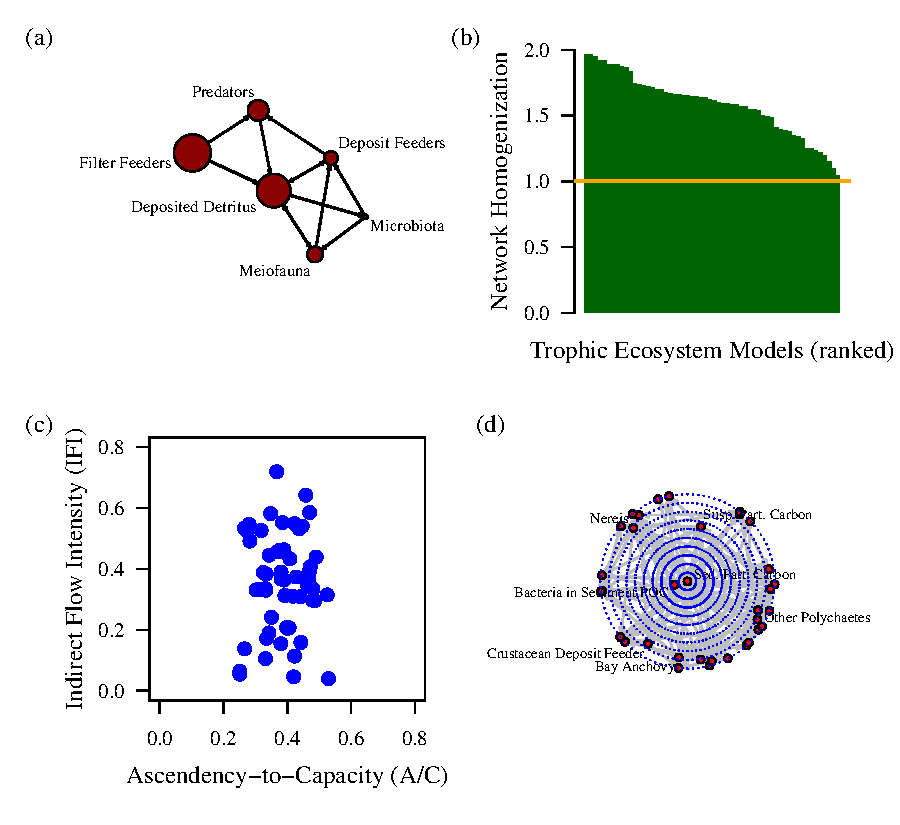
\includegraphics[scale=1]{../figures/enaR_plot_example.pdf}
\caption{Example of analysis and visualizations created with \enaR\:
  (a) network digraph of the internal flows of an oyster reef
  ecosystem model \citep{dame81}, (b) network homogenization statistic
  for 56 trophic ecosystem models (rank-ordered), (c) scatter plot
  showing the relationship between the ascendency-to-capacity ratio
  and the indirect flow index for the 56 trophic ecosystem models
  (Table~xx), and (d) target plot of the betweenness centrality from
  social network analysis calculated for the xx nodes of the
  Chesapeake Bay ecosystem model \citep{baird89}. } \label{fig:example}
\end{figure*}

\begin{figure*}[t]
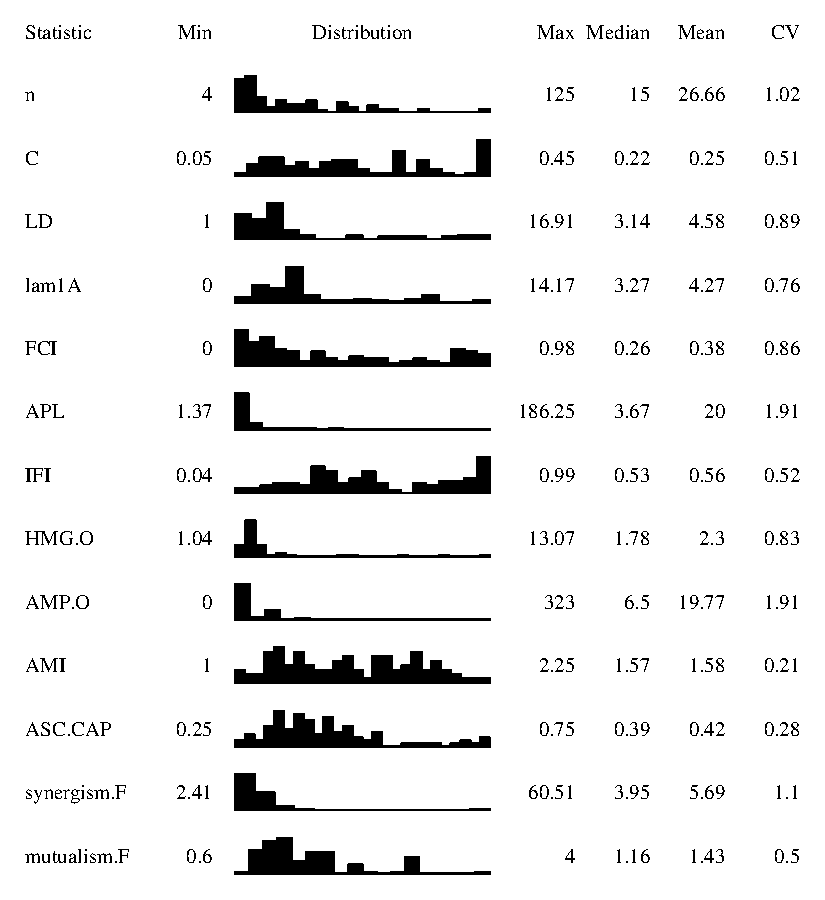
\includegraphics[scale=1]{../figures/ns_dist.pdf}
\caption{Distributions of selected ENA network statistics from to the
  100 empircially-based ecosystem models included in \enaR\ 2.0.  The
  results are summarized using a histogram showing the distribution of
  the values of each network statistic between the observed minimum
  and maximum values.  The median, mean, and coefficient of variation
  (ratio of standard deviation and mean) values are also reported.
  The network statistics are the number of nodes ($n$), the
  connectance ($C = L/n^2$), link density ($LD = L/n$), pathway
  proliferation rate (lam1A), Finn cycling index (FCI), average path
  length (APL), indirect flow intensity (IFI), output oriented network
  homogenization ratio (HMG.O), output-oriented network amplification
  ratio (AMP.O), average mutual information (AMI), the
  ascendency-to-capacity ratio (ASC.CAP), flow-based network synergism
  (synergism.F) and mutualism (mutualism.F).} \label{fig:ns}
\end{figure*}

\end{document}


